\tableofcontents
% add introduction to the table of contents and conclusion
\section{Introduction}

\subsection{Background and Motivation}

Swarm robotics is an emerging field in robotics inspired by biological systems, such as flocks of birds or colonies of ants, where simple units collaborate to achieve complex tasks. In recent years, advancements in drone technology have expanded the potential applications of swarm robotics, including environmental monitoring, search-and-rescue operations, and industrial automation \cite{swarm_survey}. In particular, drones operating as swarms offer a promising solution for tasks requiring adaptability and scalability.

One key area of interest is the integration of drone swarms into environments shared with humans. Applications such as drone-based assistance systems in healthcare, smart warehouses, and collaborative robotics emphasize the need for reliable, safe human-drone interaction \cite{swarm_survey}. The use of drones in indoor environments, where traditional positioning systems such as GPS are not viable, presents both opportunities and challenges, particularly when human safety and interaction are prioritized.

In this context, existing swarm control platforms like Crazyswarm and CFlib offer robust tools for drone coordination and control. However, these platforms often require specialized equipment, such as motion capture systems, and rely on Python-based libraries, limiting accessibility for non-expert users and those working in non-research settings \cite{crazyflie,bitcraze_cflib}. This raises a gap: a need for more accessible, intuitive control systems that allow seamless interaction between human operators and drone swarms in real-time indoor environments.

\subsection{Problem Statement}

While existing platforms provide powerful tools for swarm control, they do not address the challenge of creating a system that integrates human pose detection with real-time drone control in a user-friendly and accessible way. Most current systems are limited in their ability to allow developers to work directly with drones in environments where they need to safely interact with human operators.

This research addresses this gap by proposing a web-based platform for controlling swarms of Crazyflie drones in indoor spaces using real-time human pose estimation. The platform aims to enable intuitive and responsive interaction between humans and drones without requiring complex external systems.

We want to have our scene of drones including our operators and drones. Similarly in red is the drone system and in yellow the human system with the human pose detection. In red above there is the drone localization system. In grey above is the human localization system.

\begin{figure}[htbp]
    \centerline{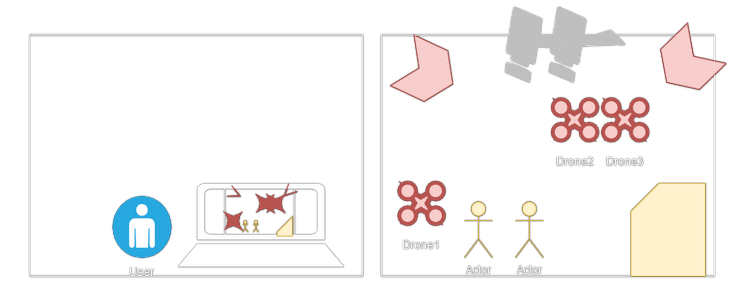
\includegraphics{images/setting.png}}
    \caption{ Our setup for controlling drones indoors around humans. Similarly in red is the drone system and in yellow the human system with the human pose detection. In red above there is the drone localization system. In grey above is the human localization system. }
    \label{fig}
    \end{figure}

\subsection{Research Objectives}

This research aims to address the limitations of existing swarm control platforms by developing a user-friendly, web-based system for controlling swarms of drones in indoor environments where interaction with humans is required. The main objectives of this research are as follows:

\begin{itemize}
    \item Develop a web-based platform for controlling swarms of Crazyflie drones, enabling easier access for developers, researchers, and non-experts.
    \item Integrate real-time human pose detection using affordable and accessible technologies, such as Intel RealSense and MediaPipe \cite{realsense_mediapipe}.
    \item Ensure safe and responsive drone interactions in indoor environments by integrating collision avoidance systems and real-time feedback.
    \item Evaluate the platform's performance in both controlled and dynamic indoor environments with human interaction.
\end{itemize}

This research will demonstrate how a web-based interface, coupled with advanced human pose detection, can make drone swarm control more accessible and enhance human-drone collaboration in shared spaces.

\subsection{Significance of the Research}

The proposed platform has the potential to significantly impact the field of swarm robotics by broadening access to swarm control technologies. Currently, systems like \textit{CrazySwarm} and \textit{CFLib} require Python-based development, which limits their use to researchers or developers with specific technical expertise \cite{crazyflie,bitcraze_cflib}. By shifting to a web-based architecture, this research will make drone control systems more accessible to a wider audience, enabling cross-platform development and more intuitive interfaces.

Furthermore, by integrating real-time human pose detection, this platform introduces a novel method for enabling drones to interact with humans safely in indoor environments. This has wide-ranging applications, from smart warehouses, where drones assist human workers \cite{flyjacket, human_drone_interaction}. The platform also has the potential to be used in educational settings, allowing students to interact with drones without complex technical setups.

Ultimately, this research fills a critical gap in current swarm robotics systems, creating a foundation for future development in both research and practical applications, particularly in areas where drone-human interaction is necessary.

\subsection{Scope and Limitations}

The proposed platform has limitations that should be considered. First, the platform is designed for indoor environments, where GPS signals are unreliable, and human interaction is a primary concern. It can not work outdoors.

The platform will not adress internal positioning of the drones, only external positioning.

The platform will not address drone swarm control in outdoor or GPS-based environments.

The platform will use real-time human pose detection technologies like Intel RealSense and MediaPipe, which may have limitations in complex environments.

Despite these limitations, the proposed platform offers a significant advancement in swarm robotics by providing a user-friendly interface for controlling drones in indoor environments around humans. The platform's focus on accessibility and safety makes it a valuable tool for researchers, developers, and educators interested in swarm robotics and human-drone interaction.

\subsection{Structure Overview}
    Chapter 1 will review the State of the Art, including existing swarm control platforms like CrazySwarm, ModQuad, and human pose detection systems.

    Chapter 2 will describe the design and implementation of the proposed Drone Control Kernel.

    Chapter 3 Will describe the integration of real-time human pose detection.

    Chapter 4 will present the platform for human-swarm interaction will present the experimental setup and results, validating the platform's functionality including possible extensions of the platform for larger-scale deployment.

    Chapter 5 will discuss the conclusions

% \subsection*{Motivation}
% \subsubsection*{Overview of Swarm Robotics}


% We present a novel platform for controlling swarms of Crazyfly drones that utilizes more user-friendly technology compared to the existing Python CFlib controller. This approach demonstrates the feasibility and potential of safely operating drones around humans in indoor environments. By leveraging accessible interfaces, our platform aims to make more accessible Human-Drone technologies using widely used web technologies.
% Swarm robotics has garnered significant attention in recent years due to its applications in environmental monitoring, agriculture, and search-and-rescue missions. Among swarm robotics, drone swarms present unique challenges and opportunities, particularly in dynamic environments such as indoor spaces where interaction with humans becomes crucial. The ability to control multiple drones simultaneously and safely around humans is essential for realizing the full potential of swarm robotics in various applications. 
% However, existing platforms for controlling drone swarms often lack the necessary integration with human interaction.

% While several platforms exist for drone swarm control, such as CrazySwarm and CFLib, none provides an accessible, web-based system for controlling swarms in indoor environments with human interaction. This gap limits the deployment of drone swarms in shared spaces such as hospitals, warehouses, or educational environments. Our platform addresses this gap by providing a user-friendly interface for controlling drone swarms around humans indoors. By leveraging web technologies, we aim to democratize drone swarm control and enable developers to create innovative applications that combine human interaction. As we are in a research environment we are able to test and develop this platform in a safe environment. We are able to test the platform with known people and subjects. We plan on testing it further and giving it to students to test further and develop on. This technology gives possibilities in development to warehouses for adding drone carriers around sensitive objects or animals.

% Our technological platform is based on the Crazyflie UAVs, which are widely used in research and educational settings due to their small size, agility, and open-source software. By developing a web-based interface for controlling these drones, we aim to lower the barrier to entry for developers and researchers interested in swarm robotics. Our platform integrates real-time human pose detection and collision avoidance to ensure safe operation of drone swarms around humans. This integration enables developers to create interactive applications that leverage human-drone interaction in indoor environments.

% For this we have 5 crazyflie drones that 


\begin{marginfigure}[-5cm] % Adjust the vertical placement
    \centering
    \includegraphics[width=\linewidth]{images/plastic-waste.png}
    \caption{Plastics pollution on a beach}
    \label{fig:plastics}
\end{marginfigure}
% annoncer le plan et resumer les parties en quelques lignes
\section{State of the Art}
% ajouter 
In recent years, swarm drone technology has advanced significantly, leading to breakthroughs in human-drone interaction and multi-robot systems. While several research efforts have focused on the safety, control, and interaction between drones and humans, there remains a gap in the availability of robust platforms for developers to control drone swarms indoors around humans. This section will explore existing works that demonstrate safe operation of drones around humans, systems that enable real-time drone control based on human input, and the identified gaps in the current technological landscape.

\subsection{Safe Drone Flight Around Humans}

Safety is a primary concern when operating drones in close proximity to humans, especially in confined spaces such as indoor environments. Several research efforts have focused on ensuring that drones can operate around humans without posing significant risks.

One such project is Drone \& Me, which investigates how drones can safely navigate around humans by recognizing human poses and responding accordingly \cite{drone_me}. In addition, Ju et al. (2017) proposed real-time trajectory adjustments for drones to ensure safe flight paths when operating around humans indoors. These systems emphasize the importance of autonomous collision avoidance and the use of protective hardware to mitigate risks \cite{ju_safety}.

\subsection{ Controlling Drones with Human Input}

Beyond safety, there has been significant progress in enabling human control over drones through various input methods, such as body gestures, hand movements, or wearable technology. The FlyJacket platform, for instance, allows a user to intuitively control a drone by wearing an exoskeleton that translates upper body movements into flight commands \cite{flyjacket}. This system demonstrates that drones can be controlled naturally and in real-time based on human gestures, but it is limited to controlling a single drone at a time.

In a more general approach, Cai et al. (2019) explored how drones can follow human postures and gestures using computer vision, allowing for more flexible interactions with drones \cite{cai_human_drone}. These systems highlight the potential for intuitive drone control but lack the scalability needed to control swarms of drones effectively.

\subsection{Technological Platforms for Swarm Drones}

Several robust platforms have been developed to enable scalable swarm drone systems. Among these, Crazyflie is a widely used platform for research on nano-quadrotor swarms. It provides the infrastructure for advanced coordination and trajectory planning of multiple drones in a shared airspace. The platform’s compatibility with tools like \gls{ROS} (Robot Operating System) makes it a flexible tool for swarm applications \cite{crazyflie}.

Another well-known platform is Kilobot, developed by Harvard’s Wyss Institute. Though primarily a ground-based swarm robotics platform, Kilobot’s decentralized control algorithms provide valuable insights into swarm intelligence and distributed behaviors, which are applicable to aerial drones as well \cite{kilobot}. ModQuad further builds on swarm modularity by allowing multiple drones to self-assemble mid-air, forming complex structures that can adapt to various tasks \cite{modquad}.

The CrazyChoir platform demonstrates how multiple Crazyflie drones can perform synchronized movements in an artistic or musical context, emphasizing scalability in both control and safety \cite{crazychoir}. These platforms provide strong technological foundations for swarm robotics, yet none fully integrate human interaction into swarm control in indoor environments.

CrazySwarm \cite{preiss2017crazyswarm} represents the current state of the art for large-scale swarm control in research environments, particularly in fields like swarm robotics, distributed systems, and human-swarm interaction. It leverages \gls{ROS} for modularity and scalability, and its integration with real-time motion capture systems provides a sophisticated platform for studying collective behaviors. Conversely, CFLib Swarm focuses on providing accessible, low-level control of Crazyflie drones for smaller-scale applications, mainly for educational purposes and basic experimentation.

CrazySwarm provides a more advanced, scalable solution for handling large swarms in complex environments. It overcomes the limitations of CFLib \cite{bitcraze_cflib} Swarm, such as lack of real-time positioning and high-level control, making it the preferred platform for research in swarm robotics.

We want to note here that in the Institute for Future Technologies there was a project that started with \gls{ROS} but had issues as \gls{ROS} adds a layer of abstraction and infrastructure that provides many advantages but also introduces overhead. \cite{carstens_intelligent_nodate}. CFLib avoids this overhead by interacting directly with the drones in a more lightweight package.

\begin{figure}[htbp]
    \centerline{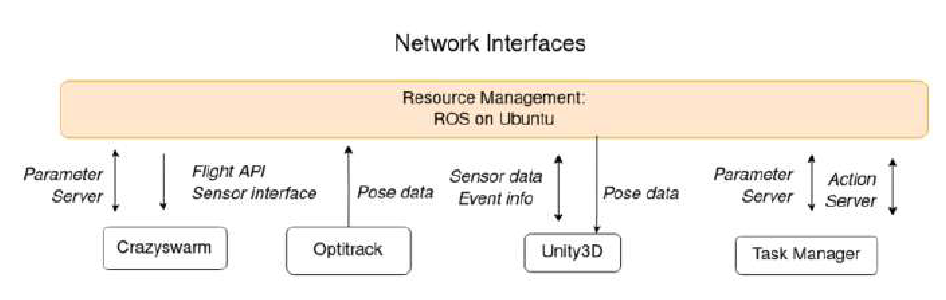
\includegraphics[width=0.5\textwidth]{images/ROSnetwork.png}}
    \caption{Drone Control Kernel developed by previous dronelab team at IFT.\cite{carstens_intelligent_nodate}}
    \label{fig}
    \end{figure} 

\subsection{Human Pose Detection for Drone Control}

Human-drone interaction has advanced with technologies that allow drones to react to human movements. One notable platform is FlyJacket, a wearable exoskeleton that translates upper body movements into drone control. FlyJacket emphasizes intuitive and immersive control, but it is focused on single-drone systems \cite{flyjacket}.

Beyond specialized wearables, recent advances in computer vision have made it possible to detect human poses and gestures without specialized hardware. Intel RealSense, combined with MediaPipe, allows real-time human pose estimation from \gls{RGB} and depth cameras. This technology can detect skeletal movements and translate them into commands for drone control \cite{realsense_mediapipe}. The system’s accuracy and low latency make it highly applicable to environments where humans and drones must coexist.

In addition, Cai et al. (2019) proposed a monocular vision system for real-time posture recognition, where drones respond dynamically to human gestures in indoor environments. This system allows for direct interaction between humans and drones but does not yet support multi-drone systems \cite{cai_human_drone}.

Leap Motion offers another avenue for gesture-based control by detecting hand and finger movements. While Leap Motion has been successfully integrated with single drones, there is still potential to expand this to swarm systems for more complex indoor tasks \cite{leap_motion}.

The paper titled \"Drone control using Kinect-based posture detection\"~\cite{realsense_mediapipe} presents a compelling approach to enhancing human-drone interaction by leveraging \gls{RGB-D} \(Red, Green, Blue-Depth\) data from the Kinect sensor. The authors demonstrate how Kinect can effectively capture real-time human poses and positions, enabling drones to respond to user gestures with a high degree of accuracy. By utilizing the depth data, the system can determine the spatial relationship between the human operator and the drone, allowing for intuitive control commands based on body movements.

This approach significantly reduces the need for additional hardware or complex controllers, as it translates natural human actions directly into drone maneuvers. The paper emphasizes that such a system can enhance the usability and accessibility of drones, particularly in indoor environments where GPS signals may be unreliable. Furthermore, the authors highlight the potential for combining this technology with other methods, such as those explored in \cite{realsense_mediapipe} and \cite{flyjacket}, to create a more robust human-drone interaction framework that addresses current limitations in the field.
% ajouter les problemes

\subsection{Gaps in Human-Swarm Interaction Platforms}
% synthese des problemes
Despite advancements in both safety mechanisms and control systems, there remains a significant gap in providing a unified platform that enables developers to control swarms of drones indoors while safely interacting with humans. Current platforms like Crazyflie and ModQuad provide scalable solutions for drone swarms but lack the necessary integration with human pose recognition and safety protocols for operating indoors around people \cite{crazyflie, modquad}. Furthermore, while platforms like FlyJacket enable human control, they focus on single-drone control, leaving a gap in swarming capabilities. 

Thus, a key challenge remains in the development of a platform that can:

    Enable real-time control of multiple drones based on human input (e.g., gestures, body movements).
    That includes real-time posture and position as all platforms do not seem to include. \cite{cflib, crazyswarm, flyjacket}
    Ensure safe flight paths in indoor environments.

    Be accessible to developers for customization and open-source integration.
        Python is accessible but we want to be able to use these drones in unity or a web service to not require client-drone connection.
	
\pagebreak
% ajouter des appindixa1 pour ajouter les traval d'Etienne Pommel en quelques paragraphes